%% fig_weilcube.tex   (generated by make_core.py; do not edit by hand)
%% The 2^{2n} = 16 monomials w^(T) at n = 2 as the vertices of the 4-cube under the linear projection e_j -> (a_j, 1): the height is |T|, edges of one direction are parallel, and the parity of |T| separates omega_1 from omega_2.
\documentclass[tikz,border=8pt]{standalone}
\usepackage{amsmath,amssymb}
\usetikzlibrary{arrows.meta,calc,decorations.pathreplacing}
%% palette.tex -- shared colour definitions for the figures
\definecolor{PInk}{RGB}{26,32,44}
\definecolor{PBlue}{RGB}{37,82,139}
\definecolor{PTeal}{RGB}{23,127,125}
\definecolor{POchre}{RGB}{193,138,44}
\definecolor{PClay}{RGB}{178,74,58}
\definecolor{PSlate}{RGB}{108,122,137}
\definecolor{PViolet}{RGB}{110,86,150}
\definecolor{WBlue}{RGB}{223,234,246}
\definecolor{WTeal}{RGB}{220,238,236}
\definecolor{WOchre}{RGB}{250,240,218}
\definecolor{WClay}{RGB}{247,229,224}
\definecolor{WSlate}{RGB}{238,241,244}
\definecolor{PMag}{RGB}{158,58,110}
\definecolor{PGrass}{RGB}{62,124,66}
\definecolor{PAmber}{RGB}{214,112,38}
\definecolor{PIndigo}{RGB}{58,64,140}
\definecolor{PRule}{RGB}{176,186,197}

%% shared macros so the standalone figures match the paper
\providecommand{\QQ}{\mathbb{Q}}
\providecommand{\ZZ}{\mathbb{Z}}
\providecommand{\RR}{\mathbb{R}}
\providecommand{\CC}{\mathbb{C}}
\providecommand{\PP}{\mathbb{P}}
\providecommand{\Kx}{K^{\times}}
\providecommand{\HW}{W}
\providecommand{\Nm}{\mathrm{N}}
\providecommand{\Hdg}{\mathrm{Hdg}}
\providecommand{\NS}{\mathrm{NS}}
\providecommand{\cA}{\mathcal{A}}
\providecommand{\cD}{\mathcal{D}}
\providecommand{\cF}{\mathcal{F}}
\providecommand{\cP}{\mathcal{P}}
\providecommand{\cO}{\mathcal{O}}
\providecommand{\cQ}{\mathcal{Q}}
\providecommand{\bbar}[1]{\overline{#1}}
\providecommand{\ch}{\operatorname{ch}}
\providecommand{\End}{\mathrm{End}}
\providecommand{\Ext}{\operatorname{Ext}}
\providecommand{\Supp}{\operatorname{Supp}}

\begin{document}
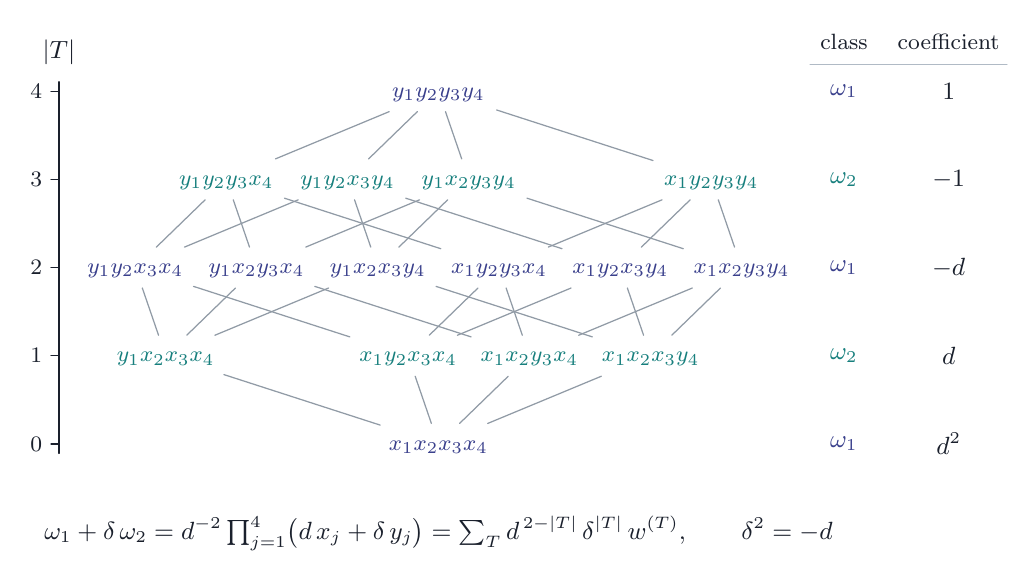
\begin{tikzpicture}[x=1cm,y=1cm,line join=round,line cap=round,
  font=\small,text=PInk,lbl/.style={inner sep=1pt}]
  \draw[PSlate!75,line width=0.45pt] (-0.7400,0.2392) -- (-2.7250,0.8808);
  \draw[PSlate!75,line width=0.45pt] (-0.0894,0.2600) -- (-0.2956,0.8600);
  \draw[PSlate!75,line width=0.45pt] (0.2681,0.2600) -- (0.8869,0.8600);
  \draw[PSlate!75,line width=0.45pt] (0.6256,0.2600) -- (2.0694,0.8600);
  \draw[PSlate!75,line width=0.45pt] (-3.5544,1.3800) -- (-3.7606,1.9800);
  \draw[PSlate!75,line width=0.45pt] (-3.1969,1.3800) -- (-2.5781,1.9800);
  \draw[PSlate!75,line width=0.45pt] (-2.8394,1.3800) -- (-1.3956,1.9800);
  \draw[PSlate!75,line width=0.45pt] (-1.1250,1.3592) -- (-3.1100,2.0008);
  \draw[PSlate!75,line width=0.45pt] (-0.1169,1.3800) -- (0.5019,1.9800);
  \draw[PSlate!75,line width=0.45pt] (0.2406,1.3800) -- (1.6844,1.9800);
  \draw[PSlate!75,line width=0.45pt] (-3.5819,2.5000) -- (-2.9631,3.1000);
  \draw[PSlate!75,line width=0.45pt] (-3.2244,2.5000) -- (-1.7806,3.1000);
  \draw[PSlate!75,line width=0.45pt] (0.4150,1.3592) -- (-1.5700,2.0008);
  \draw[PSlate!75,line width=0.45pt] (1.0656,1.3800) -- (0.8594,1.9800);
  \draw[PSlate!75,line width=0.45pt] (1.7806,1.3800) -- (3.2244,1.9800);
  \draw[PSlate!75,line width=0.45pt] (-2.3994,2.5000) -- (-2.6056,3.1000);
  \draw[PSlate!75,line width=0.45pt] (-1.6844,2.5000) -- (-0.2406,3.1000);
  \draw[PSlate!75,line width=0.45pt] (0.0300,2.4792) -- (-1.9550,3.1208);
  \draw[PSlate!75,line width=0.45pt] (1.3956,2.5000) -- (2.8394,3.1000);
  \draw[PSlate!75,line width=0.45pt] (-2.0694,3.6200) -- (-0.6256,4.2200);
  \draw[PSlate!75,line width=0.45pt] (1.9550,1.3592) -- (-0.0300,2.0008);
  \draw[PSlate!75,line width=0.45pt] (2.6056,1.3800) -- (2.3994,1.9800);
  \draw[PSlate!75,line width=0.45pt] (2.9631,1.3800) -- (3.5819,1.9800);
  \draw[PSlate!75,line width=0.45pt] (-0.8594,2.5000) -- (-1.0656,3.1000);
  \draw[PSlate!75,line width=0.45pt] (-0.5019,2.5000) -- (0.1169,3.1000);
  \draw[PSlate!75,line width=0.45pt] (1.5700,2.4792) -- (-0.4150,3.1208);
  \draw[PSlate!75,line width=0.45pt] (2.5781,2.5000) -- (3.1969,3.1000);
  \draw[PSlate!75,line width=0.45pt] (-0.8869,3.6200) -- (-0.2681,4.2200);
  \draw[PSlate!75,line width=0.45pt] (3.1100,2.4792) -- (1.1250,3.1208);
  \draw[PSlate!75,line width=0.45pt] (3.7606,2.5000) -- (3.5544,3.1000);
  \draw[PSlate!75,line width=0.45pt] (0.2956,3.6200) -- (0.0894,4.2200);
  \draw[PSlate!75,line width=0.45pt] (2.7250,3.5992) -- (0.7400,4.2408);
  \draw[PInk,line width=0.45pt] (-4.8200,-0.1200) -- (-4.8200,4.6000);
  \draw[PInk,line width=0.45pt] (-4.9200,0.0000) -- (-4.8200,0.0000);
  \draw[PInk,line width=0.45pt] (-4.9200,1.1200) -- (-4.8200,1.1200);
  \draw[PInk,line width=0.45pt] (-4.9200,2.2400) -- (-4.8200,2.2400);
  \draw[PInk,line width=0.45pt] (-4.9200,3.3600) -- (-4.8200,3.3600);
  \draw[PInk,line width=0.45pt] (-4.9200,4.4800) -- (-4.8200,4.4800);
  \draw[PRule,line width=0.45pt] (4.7200,4.8200) -- (7.2200,4.8200);
  \node[lbl,text=PIndigo,font=\footnotesize,text height=1.5ex,text depth=0.45ex] at (0.0000,0.0000) {$x_{1}x_{2}x_{3}x_{4}$};
  \node[lbl,text=PTeal,font=\footnotesize,text height=1.5ex,text depth=0.45ex] at (-3.4650,1.1200) {$y_{1}x_{2}x_{3}x_{4}$};
  \node[lbl,text=PTeal,font=\footnotesize,text height=1.5ex,text depth=0.45ex] at (-0.3850,1.1200) {$x_{1}y_{2}x_{3}x_{4}$};
  \node[lbl,text=PIndigo,font=\footnotesize,text height=1.5ex,text depth=0.45ex] at (-3.8500,2.2400) {$y_{1}y_{2}x_{3}x_{4}$};
  \node[lbl,text=PTeal,font=\footnotesize,text height=1.5ex,text depth=0.45ex] at (1.1550,1.1200) {$x_{1}x_{2}y_{3}x_{4}$};
  \node[lbl,text=PIndigo,font=\footnotesize,text height=1.5ex,text depth=0.45ex] at (-2.3100,2.2400) {$y_{1}x_{2}y_{3}x_{4}$};
  \node[lbl,text=PIndigo,font=\footnotesize,text height=1.5ex,text depth=0.45ex] at (0.7700,2.2400) {$x_{1}y_{2}y_{3}x_{4}$};
  \node[lbl,text=PTeal,font=\footnotesize,text height=1.5ex,text depth=0.45ex] at (-2.6950,3.3600) {$y_{1}y_{2}y_{3}x_{4}$};
  \node[lbl,text=PTeal,font=\footnotesize,text height=1.5ex,text depth=0.45ex] at (2.6950,1.1200) {$x_{1}x_{2}x_{3}y_{4}$};
  \node[lbl,text=PIndigo,font=\footnotesize,text height=1.5ex,text depth=0.45ex] at (-0.7700,2.2400) {$y_{1}x_{2}x_{3}y_{4}$};
  \node[lbl,text=PIndigo,font=\footnotesize,text height=1.5ex,text depth=0.45ex] at (2.3100,2.2400) {$x_{1}y_{2}x_{3}y_{4}$};
  \node[lbl,text=PTeal,font=\footnotesize,text height=1.5ex,text depth=0.45ex] at (-1.1550,3.3600) {$y_{1}y_{2}x_{3}y_{4}$};
  \node[lbl,text=PIndigo,font=\footnotesize,text height=1.5ex,text depth=0.45ex] at (3.8500,2.2400) {$x_{1}x_{2}y_{3}y_{4}$};
  \node[lbl,text=PTeal,font=\footnotesize,text height=1.5ex,text depth=0.45ex] at (0.3850,3.3600) {$y_{1}x_{2}y_{3}y_{4}$};
  \node[lbl,text=PTeal,font=\footnotesize,text height=1.5ex,text depth=0.45ex] at (3.4650,3.3600) {$x_{1}y_{2}y_{3}y_{4}$};
  \node[lbl,text=PIndigo,font=\footnotesize,text height=1.5ex,text depth=0.45ex] at (0.0000,4.4800) {$y_{1}y_{2}y_{3}y_{4}$};
  \node[lbl,anchor=east,text=PInk,font=\footnotesize] at (-4.9900,0.0000) {$0$};
  \node[lbl,anchor=east,text=PInk,font=\footnotesize] at (-4.9900,1.1200) {$1$};
  \node[lbl,anchor=east,text=PInk,font=\footnotesize] at (-4.9900,2.2400) {$2$};
  \node[lbl,anchor=east,text=PInk,font=\footnotesize] at (-4.9900,3.3600) {$3$};
  \node[lbl,anchor=east,text=PInk,font=\footnotesize] at (-4.9900,4.4800) {$4$};
  \node[lbl,anchor=south,text=PInk] at (-4.8200,4.7800) {$\lvert T\rvert$};
  \node[lbl,text=PIndigo] at (5.1500,0.0000) {$\omega_{1}$};
  \node[lbl,text=PInk] at (6.4800,0.0000) {$d^{2}$};
  \node[lbl,text=PTeal] at (5.1500,1.1200) {$\omega_{2}$};
  \node[lbl,text=PInk] at (6.4800,1.1200) {$d$};
  \node[lbl,text=PIndigo] at (5.1500,2.2400) {$\omega_{1}$};
  \node[lbl,text=PInk] at (6.4800,2.2400) {$-d$};
  \node[lbl,text=PTeal] at (5.1500,3.3600) {$\omega_{2}$};
  \node[lbl,text=PInk] at (6.4800,3.3600) {$-1$};
  \node[lbl,text=PIndigo] at (5.1500,4.4800) {$\omega_{1}$};
  \node[lbl,text=PInk] at (6.4800,4.4800) {$1$};
  \node[lbl,text=PInk,font=\footnotesize,text height=1.6ex,text depth=0.4ex] at (5.1500,5.1000) {class};
  \node[lbl,text=PInk,font=\footnotesize,text height=1.6ex,text depth=0.4ex] at (6.4800,5.1000) {coefficient};
  \node[lbl,anchor=north,text=PInk] at (0.0000,-0.8800) {$\omega_{1}+\delta\,\omega_{2}=d^{-2}\prod_{j=1}^{4}\bigl(d\,x_{j}+\delta\,y_{j}\bigr)=\sum_{T}d^{\,2-\lvert T\rvert}\,\delta^{\lvert T\rvert}\,w^{(T)},\qquad \delta^{2}=-d$};
\end{tikzpicture}
\end{document}
